
\newcommand{\Uoc}{U_{\text{OC}}}
\newcommand{\jsc}{j_{\text{SC}}}
\newcommand{\Pmax}{P_{\text{max}}}
\newcommand{\meann}[1]{\langle #1 \rangle_n}

\section{Characterization of the I-V-Curves}\label{sec:charac}

In order to characterize the manufactured solar cells, we connected them to a multimeter and put them on top of a solar simulator. The simulator utilizes the AM 1.5 global reference spectrum and is also outfitted with 5 different filters to dim the light. Using the multimeter we applied a sequence of voltages to the cell and measured the current that was produced as a result. This was done at different levels of intensity of the light and in the dark.\\
In order to get an accurate measure for the intensity with which the solar simulator irradiated the cells, we \textbf{more stuff to write here}\\
In order to calculate the open circuit voltage $\Uoc$ and the short circuit current density $\jsc$ for a set of measurements, we did a linear interpolation between the two closest points to the relevant axis ($j$-axis for $\Uoc$, $U$-axis for $\jsc$), on each side of it. So if our chosen points for the calculation of $\Uoc$ are $\{(j_1,U_1),(j_2,U_2)\}$ and for $\jsc$ are $\{(j_1^\prime,U_1^\prime),(j_2^\prime,U_2^\prime)\}$, then the formulas for $\Uoc$ and $\jsc$ are as follows.

\begin{align}
\Uoc &= \frac{U_2 j_1 - U_1 j_2}{j_1-j_2}\\
\jsc &= \frac{U_1^\prime j_2^\prime - U_2^\prime j_1^\prime}{U_1^\prime-U_2^\prime}
\end{align}

To get the maximum power density we simply multiplied the current densities and voltages and took the largest value.

\begin{align}
\Pmax = \max_{i} j_i\cdot U_i
\end{align}

The fill factor $FF$ is defined as the ratio of maximum power to the product of open circuit voltage and short circuit current.

\begin{align}
FF = \frac{\Pmax}{\Uoc \cdot \jsc}
\end{align}

In the case of sets $\mathbb{S}_3$ and $\mathbb{S}_\star$ we had multiple working cells. For these we decided to do all calculation with the mean of the current density over the working cells $n$ and include the standard deviation in the uncertainties of our results. The systematic errors of the current $u_{I,\text{sys}}$ and voltage $u_{U,\text{sys}}$ measurements were taken from \cite{keithley}. The uncertainty of the mean of the current density of measurement pair $p$ then is given as:

\begin{align}
u_{\meann{j_p}} = \sqrt{\frac{\sigma_{j,p}^2}{N} + \meann{u_{j_p,\text{sys}}}^2}
\end{align}

With sample size $N$ being the amount of working cells of the set and the systematic error:

\begin{align}
u_{j_{pn},\text{sys}} = \sqrt{ \left( \frac{ u_{I_{pn},\text{sys}}}{A_n}\right)^2+\left( j_{pn}\frac{u_{A_n}}{A_n} \right)^2}
\end{align}

The uncertainty of maximum power and fill factor, as well as short circuit current and open circuit voltage can then be obtained through Gaußian error propagation.

\subsection{First set of \BHSC s}

For the first set of \BHSC s $\mathbb{S}_1$, for which only one cell was not shorted, we obtained the following parameters.

\begin{figure}[h]\centering
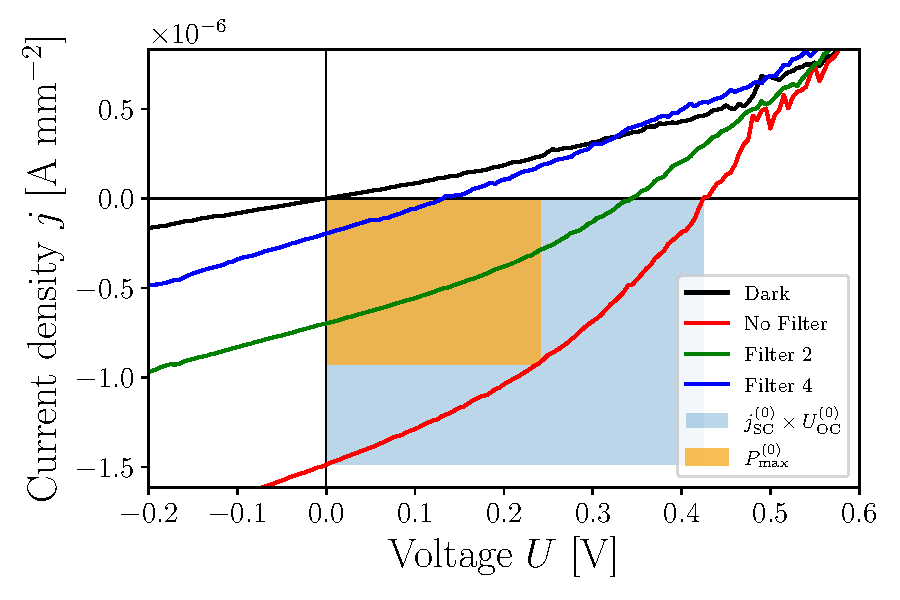
\includegraphics[width=\columnwidth]{../../../IV-Curve-Analysis/OSC1Graph.pdf}
\caption{Current density measurements for the first architecture}
\label{fig:OSC1Graph}
\end{figure}

\subsection{Third set of \BHSC s}

\begin{table}[h]\centering
\caption{Key parameters for each set of \BHSC s}
\label{tab:keyparams}
\begin{tabular}{@{}cccccc@{}}\toprule
Filter $i$ & $S_i$ & $\Pmax$ [$\mu$W cm$^{-2}$] & $\Uoc$ & $\jsc$ & $FF$\\\midrule
0 & - & $  \pm  $ & $  \pm  $ & $  \pm  $ & $  \pm  $ \\
1 & - & $  \pm  $ & $  \pm  $ & $  \pm  $ & $  \pm  $ \\
2 & - & $  \pm  $ & $  \pm  $ & $  \pm  $ & $  \pm  $ \\
3 & - & $  \pm  $ & $  \pm  $ & $  \pm  $ & $  \pm  $ \\
4 & - & $  \pm  $ & $  \pm  $ & $  \pm  $ & $  \pm  $ \\
5 & - & $  \pm  $ & $  \pm  $ & $  \pm  $ & $  \pm  $ \\\bottomrule
\end{tabular}
\end{table}

